%%%%%%%%%%%%%%%%%%%%%%%%%%%%%%%%%%%%%%
% LaTeX poster template
% Created by Nathaniel Johnston
% August 2009
% http://www.nathanieljohnston.com/2009/08/latex-poster-template/
%%%%%%%%%%%%%%%%%%%%%%%%%%%%%%%%%%%%%%

\documentclass[final]{beamer}
\usepackage[scale=0.8,orientation=landscape,size=a0]{beamerposter}
\usepackage{graphicx} % allows us to import images

%-----------------------------------------------------------
% Define the column width and poster size
% To set effective sepwid, onecolwid and twocolwid values, first choose how many columns you want and how much separation you want between columns
% The separation I chose is 0.024 and I want 4 columns
% Then set onecolwid to be (1-(3+1)*0.02)/3 = 0.307
% Set twocolwid to be 2*onecolwid + sepwid = 0.613
%-----------------------------------------------------------

\newlength{\sepwid}
\newlength{\onecolwid}
\newlength{\twocolwid}
\newlength{\threecolwid}
\setlength{\sepwid}{0.02\paperwidth}
\setlength{\onecolwid}{0.307\paperwidth}
\setlength{\topmargin}{-0.7in}
\usetheme{confposter}
\usepackage{exscale}
\usepackage{amsmath}
\usepackage{amssymb}
\usepackage{bm}
\usepackage{pgfplots}
\usepackage{array}
%\usepackage{natbib}
\usepackage{sidecap}
\usepackage{subfigure}
\usepackage{graphicx}

\newcommand{\argmax}{ \operatorname*{arg \max}}
\newcommand{\argmin}{ \operatorname*{arg \min}}
\newcommand{\x}{\mathbf{x}}
\newcommand{\pair}{(\x,\x')}
\newcommand{\param}{\bm{\theta}}
\newcommand{\X}{\mathbf{X}}
\newcommand{\y}{y}
\newcommand{\data}{\mathcal{D}}
\newcommand{\h}{\mathbf{H}}
\newcommand{\g}{\mathbf{G}}
\newcommand{\w}{\mathbf{W}}
\newcommand{\pr}{\mathrm{P}}
\newcommand{\ent}{\mathrm{H}}
\newcommand{\info}{\mathrm{I}}
\newcommand{\E}{\mathbb{E}}
\newcommand{\T}{\mathrm{T}}
\newcommand{\ie}{i.\,e.\ }
\newcommand{\eg}{e.\,g.\ }
\newcommand{\latfun}{f}
 \newcommand{\List}{\mathcal{L}}


\definecolor{mycolor1}{rgb}{0.8,0.8,0}
\definecolor{mycolor2}{rgb}{0,1,1}
\definecolor{mycolor3}{rgb}{1,0,1}
\definecolor{mycolor4}{rgb}{1,0.8,0.5}
\definecolor{mycolor5}{rgb}{0.7,0.4,0.01}

%-----------------------------------------------------------
% The next part fixes a problem with figure numbering. Thanks Nishan!
% When including a figure in your poster, be sure that the commands are typed in the following order:
% \begin{figure}
% \includegraphics[...]{...}
% \caption{...}
% \end{figure}
% That is, put the \caption after the \includegraphics
%-----------------------------------------------------------

\usecaptiontemplate{
\small
\structure{\insertcaptionname~\insertcaptionnumber:}
\insertcaption}

%-----------------------------------------------------------
% Define colours (see beamerthemeconfposter.sty to change these colour definitions)
%-----------------------------------------------------------

\setbeamercolor{block title}{fg=blue,bg=white}
\setbeamercolor{block body}{fg=black,bg=white}
\setbeamercolor{block alerted title}{fg=white,bg=dblue!70}
\setbeamercolor{block alerted body}{fg=black,bg=dblue!10}

%-----------------------------------------------------------
% Name and authors of poster/paper/research
%-----------------------------------------------------------

\title{Collaborative Gaussian Processes for Preference Learning}
\author{Neil Houlsby, Jose Miguel Hern\'{a}ndez-Lobato, Ferenc Husz\'{a}r, Zoubin Ghahramani}
\institute{Computational and Biological Learning Lab, Department of Engineering, University of Cambridge}

%-----------------------------------------------------------
% Start the poster itself
%-----------------------------------------------------------

\begin{document}

\begin{frame}[t]
  \begin{columns}[t]

  \begin{column}{\sepwid}\end{column}         % empty spacer column

  \begin{column}{\onecolwid}

    \begin{block}{Multi-user Preference Learning}
        \begin{itemize}
          \item General approach: model a user with a latent `utility' function $f(\x_i)>f(\x_j)$ indicated item $i$
            is preferred to item $j$.
          \item Gaussian process models are popular for \emph{single-user} preference learning
            \cite{chu2005}.
          \item Multiple users: leverage shared behavior.
          \item May or may not have \emph{useful} features for the users.
          \item Current approaches require solving at least $U$ ($=$ number of users) Gaussian processes \cite{bonilla2010, birlutiu2009}.
        \end{itemize}
      \end{block}

    \begin{alertblock}{The Task}
      \begin{itemize}
        \item {\bf Goal}: Build a scalable multi-user probabilistic preference learner that
            may incorporate features if available (and useful).
        \item {\bf Approach}: Combine dimensionality reducing methods of collaborative filtering.
          with flexible Gaussian process preference function modeling.
        \item {\bf Further desiderata}: Efficient inference with preference data, `active sampling' of item pairs for efficient data collection.
      \end{itemize}
    \end{alertblock}

      \begin{block}{Reformulating Preference Learning as Binary Classification}
      \begin{itemize}
        \item Let $ \mathbf{x}\in\mathcal{X}$ denote the item features vectors, and
        $y\in\{-1,+1\}$ the preference labels.
        $ f:\mathcal{X}\mapsto\mathbb{R}$ is a user's `preference' or utility function.
        GP preference learning \cite{chu2005}:
        \begin{align}
          \mathcal{P}(y|\mathbf{x}_i,\mathbf{x}_j,f) &= \Phi[(f[\mathbf{x}_i] -
            f[\mathbf{x}_j])y]\,, \notag
        \end{align}
        where $\Phi = \text{Gaussian c.d.f}\,.$
        \item Define $g:\mathcal{X}^2\mapsto \mathbb{R}$ as $g(\x_i, \x_j) = f(\x_i) - f(\x_j)$, now
        \begin{align}
          \mathcal{P}(y|\mathbf{x}_i,\mathbf{x}_j,g) &= \Phi[g(\mathbf{x}_i,
          \mathbf{x}_j)y]\,. \notag
        \end{align}
        \item GP prior on $f$ and a linear operation $\rightarrow$ GP on $g$; derive the \emph{preference
          kernel}:
          \begin{align}
            k_\text{pref}((\x_i,\x_j),(\x_k,\x_l)) = k(\x_i,\x_k) + k(\x_j,\x_l) - k(\x_i,\x_l) -
            k(\x_j,\x_k)\,.\notag
          \end{align}
        \item Puts all \emph{anti-symmetry} constraints into the prior, also respects \emph{transitivity}.
        \item This kernel greatly simplifies the inference algorithm.
        \end{itemize}
      \end{block}

      \begin{block}{Active Sampling of Item Pairs}
      \begin{figure}
        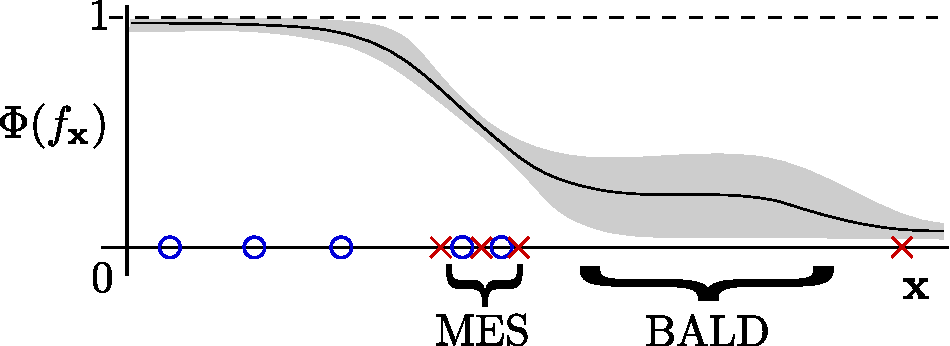
\includegraphics[scale = 1.0]{figs/BALD_eg.pdf}
        \caption{Toy example with 1D input. Circles and crosses
        denote labelled data. The plot shows the mean and variance of the GP predictive
        distribution. Maximum Entropy Sampling (MES)
        samples from the region of highest marginal uncertainty, ignoring the
        second term in \eqref{eq:bald2}. BALD samples
        from the region of greatest uncertainty in the latent function.\label{fig:bald}}
      \end{figure}
      \begin{itemize}
        \item Classic objective \cite{lindley1956}, minimize the entropy $\ent[\mathcal{P}]$
        of the posterior over the parameters:
        \begin{equation}
          \ent[\mathcal{P}(g|\mathcal{D})] - \E_{\mathcal{P}(y|\mathbf{x}_i,\mathbf{x}_j,\data)}
          \left[ \ent[\mathcal{P}(g|y,\mathbf{x}_i,\mathbf{x}_j,\data)]\right]\,. \label{eq:bald1}
        \end{equation}
        \item Problems:
        \begin{enumerate}
          \item Computational: large number of posterior updates required, $2n$ where $n=$ number of unseen pairs.
          \item Intractable: entropy of high dimensional parameter spaces hard to compute,
          approximations (e.g. Laplace) required for GPs.
        \end{enumerate}
        \item Solution: rearrange to the following formulation:
          \begin{align}
            \ent[\mathcal{P}(y|\mathbf{x}_i,\mathbf{x}_j,\data)] - \E_{\mathcal{P}(g|\data)}
            \left[\ent\left[ \mathcal{P}(y|\mathbf{x}_i,\mathbf{x}_j,g)\right]\right]\,.
            \label{eq:bald2}
          \end{align}
        \item We call this objected \emph{Bayesian Active Learning with Disagreement}.
        \item \eqref{eq:bald2} requires only $1$ posterior update, and Bernoulli entropies only.
        \item First term yields `Maximum Entropy Sampling' \cite{sebastiani2000}, the second
        discourages locations of inherent uncertainty, see Fig. \ref{fig:bald}.
        \item With a Gaussian approximation to the posterior (EP, Laplace) for a model with a GP
        prior on $g$ and Probit likelihood function (exploiting the preference kernel)
        \eqref{eq:bald2} becomes:
        \begin{equation}
        \mathrm{h} \left[ \Phi\left( \mu_{\x}(\sigma^2_{\x} + 1)^{-1/2} \right)\right] -
        C(\sigma_{\x}^2 + C^2)^{-1/2} \exp\left(-\mu_{\x}^2(2\left(\sigma_{\x}^2 +
        C^2\right))^{-1}\right)\,.\notag
        \end{equation}
        where $h[f] = -f\log f - (1-f)\log(1-f)$ and $C=\sqrt{\pi\log 2 / 2}$.
      \end{itemize}
      \end{block}

    \end{column}

    \begin{column}{\sepwid}\end{column} % empty spacer column

    \begin{column}{\onecolwid}

      \begin{alertblock}{The Model - Collaborative Gaussian Processes}
        \begin{itemize}
          \item Introduce a set of `shared latent functions':
            $\mathbf{H} = \{h_1\ldots h_D\}$, $D \ll U$.
          \item For the $u$-th user, construct their `user latent function':
            \begin{equation}
              g_{u}(\mathbf{x}_j,\mathbf{x}_k)=\sum_{d=1}^{D}w_{u,d}h_{d}
                (\mathbf{x}_j,\mathbf{x}_k)\,.\notag
            \end{equation}
          \item $\mathbf{W} = \{\{w_{u, d}\}_{u=1}^U\}_{d=1}^D$ are the user-specific weights.
          If user features are available
            $\mathbf{U} = \{\mathbf{u}_1\ \ldots \mathbf{u}_U\}$ replace these with functions:
            $w_d(\mathbf{u})$.
        \end{itemize}
      \end{alertblock}

      \begin{block}{Bayesian Formulation}
        \begin{itemize}
          \item Likelihood function uses the Probit function:
            \begin{align*}
              \mathcal{P}(\mathbf{T}^{(\mathcal{D})}|\mathbf{G}^{(\mathcal{D})})
              = \prod_{u=1}^U \prod_{i=1}^{M_u} \Phi[t_{u,z_{u,i}}
              g_{u,z_{u,i}}]\,.
            \end{align*}
        \item GP priors on `shared latent functions' and weights:
          \begin{equation}
            \mathcal{P}(\mathbf{H}|\mathbf{X},\List) =
            \prod_{j=1}^{D}\mathcal{N}(\mathbf{h}_j|\mathbf{0},\mathbf{K}_\text{items})\,,\qquad
            \mathcal{P}(\mathbf{W}|\mathbf{U}) =
            \prod_{d=1}^D
            \mathcal{N}(\mathbf{w}_{\cdot,d}|\mathbf{0},\mathbf{K}_\text{users})\,.\notag
          \end{equation}
        \item Enforce consistency in the matrix factorization:
          \begin{equation*}
            \mathcal{P}(\mathbf{G}^{(\mathcal{D})}|\mathbf{W},\mathbf{H}) =
            \prod_{u=1}^{U}
            \prod_{i=1}^{M_u}\delta[g_{u,z_{u,i}}-\mathbf{w}_u\mathbf{h}_{\cdot,z_{u,i}}]\,.
          \end{equation*}
       \end{itemize}

       \begin{figure}[h!]
       \centering
       \begin{tabular}{l}
       \hskip0.0\linewidth 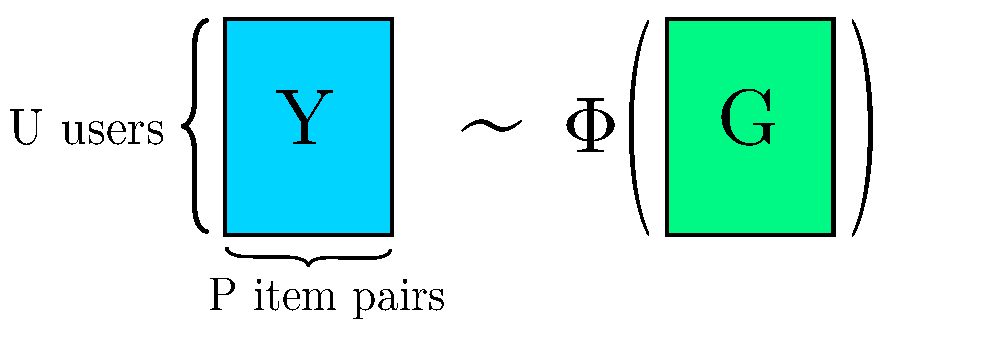
\includegraphics[scale=1.0]{figs/CPmatrices1.pdf} \\
       \hskip0.1\linewidth 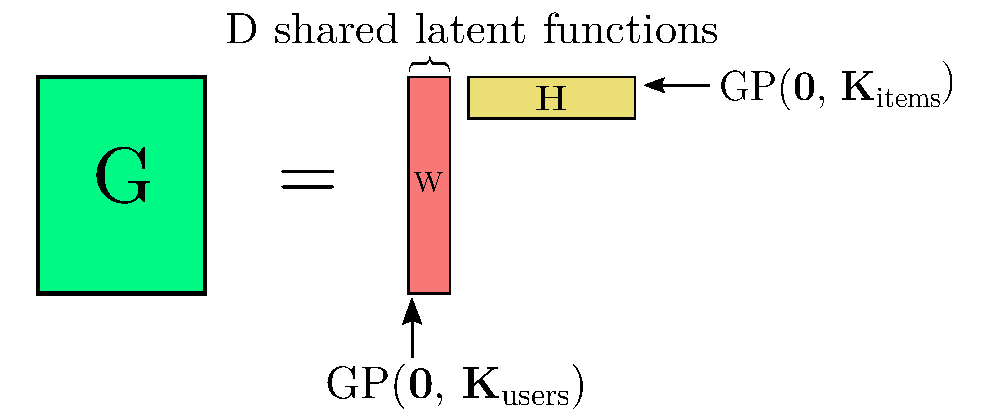
\includegraphics[scale=1.0]{figs/CPmatrices2.pdf}
       \end{tabular}
        \caption{Graphical depiction of the matrices used in the proposed model.}
       \end{figure}

       \begin{table}
       \caption{Notation}
       \begin{tabular}{l|l}
       $\mathcal{L}$ & List of $P$ item pairs evaluated by users. \\
       $\mathcal{D}$ & Indices of particular items in $\mathcal{L}$ evaluated by each
         user. \\
       $\mathbf{X}, \mathbf{U}$  & Set of item and user feature vectors respectively. \\
       $\mathbf{T}^{(\mathcal{D})}\in \{-1,+1\}^{U\times P}$ &
         Matrix of preference evaluations corresponding to items in $\mathcal{D}$. \\
       $\mathbf{G}^{(\mathcal{D})}\in \mathbb{R}^{U\times P}$ &
         Matrix of `user preference functions'. \\
       $\mathbf{H}\in \mathbb{R}^{D\times P}$ & Matrix of `shared preference functions'. \\
       $\mathbf{W}\in \mathbb{R}^{U\times D}$ & Matrix of user weights.
       \end{tabular}
       \end{table}
    \end{block}

    \begin{block}{Inference}
       \begin{itemize}
         \item Hybrid scheme: combine Expectation Propagation and Variational Bayes.
         \item Approximate the posterior with a fully factorised product of Gaussians $Q$:
           \begin{align*}
            \overbrace{\mathcal{P}(\mathbf{W},\mathbf{H},\mathbf{G}^{(\mathcal{D})}
            |\mathbf{T}^{(\mathcal{D})},\mathbf{X},\List)}^{\text{posterior distribution}}
            &=
            \frac{\overbrace{\mathcal{P}(\mathbf{T}^{(\mathcal{D})}|\mathbf{G}^{(\mathcal{D})})}^{f_1}
            \overbrace{\mathcal{P}(\mathbf{G}^{(\mathcal{D})}|\mathbf{W},\mathbf{H})}^{f_2}
            \overbrace{\mathcal{P}(\mathbf{W}|\mathbf{U})}^{f_3}
            \overbrace{\mathcal{P}(\mathbf{H}|\mathbf{X},\List)}^{f_4}}
            {\mathcal{P}(\mathbf{T}^{(\mathcal{D}}|\mathbf{X},\List)}\,.\\
            \approx \mathcal{Q}(\mathbf{W},\mathbf{H},\mathbf{G}^{(D)}) &=
            \prod_{i=1}^4 \hat{f}_i(\mathbf{W}, \mathbf{H}, \mathbf{G}^{(D)})\,.
          \end{align*}
          \item Iteratively refine $\hat{f}_1,\hat{f}_3,\hat{f_4}$ with EP i.e. minimize
            $\mathrm{KL}(\mathcal{Q}^{\setminus i}f_i||)\mathcal{Q}^{\setminus i}\hat{f}_i$ with respect
            to the parameters.
          \item Refine $\hat{f}_2$ (the matrix factorization) with VB i.e. reverse the direction of
            the KL.
        \end{itemize}
      \end{block}

    \end{column}

      \begin{column}{\sepwid}\end{column}   % empty spacer column

      \begin{column}{\onecolwid}

        \begin{block}{Small Scale Experiments}
          \begin{table}[h!]
          \centering
          \caption{Related algorithms and their computational complexities.}
          \begin{tabular}{l|l|l}
            Notation &  Algorithm & Complexity of Inference \\ \hline
            {\bf CPU} & Collaborative Preference (with user features) & $\mathcal{O}(DU^3+DP^3+D\sum_u
            N_u)$  \\
            {\bf CP} & Collaborative Preference (without user features) & $\mathcal{O}(DP^3+D\sum_u
            N_u)$\\
            {\bf Bi} & \cite{birlutiu2009} & $\mathcal{O}(UP^3)$\\
            {\bf Bo} & \cite{bonilla2010} & $\mathcal{O}((\sum_{u=1}^U N_u)^3)$  \\
            {\bf SU} & Single-user \cite{chu2005} & $\mathcal{O}(UP^3)$
          \end{tabular}
          \end{table}

          \vskip-0.5cm
          %\renewcommand{\arraystretch}{0.9}
\newcommand{\ic}{\hspace{0.25cm}}
\begin{table}
\begin{minipage}[b]{0.49\columnwidth}
\centering
\caption{Average test error with 100 users.}
\resizebox{0.9 \columnwidth}{!}{
\begin{tabular}{@{\ic}l@{\ic}c@{\ic}c@{\ic}c@{\ic}c@{\ic}c@{\ic}c@{\ic}}
\hline
\textbf{Dataset} &\textbf{CPU}&\textbf{CP}&\textbf{BI}&\textbf{BO}&\textbf{SU}\\
\hline
Synthetic&0.162&0.180&0.175&\bf{0.157}&0.226\\
Sushi&0.171&0.163&\bf{0.160}&0.266&0.187\\
MovieLens&0.182&\bf{0.166}&0.168&0.302&0.217\\
Election&0.199&0.123&\bf{0.077}&0.401&0.300\\
Jura&0.159&\bf{0.153}&\bf{0.153}&0.254&0.181\\
\hline
\end{tabular} \label{tab:errorSmallDatasets}
}
\end{minipage}
\begin{minipage}[b]{0.5\columnwidth}
\centering
\caption{Training times (s) with 100 users.}
\resizebox{0.9 \columnwidth}{!}{
\begin{tabular}{@{\ic}l@{\ic}r@{\ic}r@{\ic}r@{\ic}r@{\ic}r@{\ic}r@{\ic}}
\hline
\textbf{Dataset} &\textbf{CPU}&\textbf{CP}&\textbf{BI}&\textbf{BO}&\textbf{SU}\\
\hline
Synthetic&7.793&9.498&22.524&311.574&0.927\\
Sushi&5.694&4.307&20.028&215.136&0.817\\
MovieLens&5.313&4.013&19.366&69.048&0.604\\
Election&13.134&12.408&20.880&120.011&0.888\\
Jura&3.762&2.404&15.234&88.502&0.628\\
\hline
\end{tabular} \label{tab:timeSmallDatasets}
}
\end{minipage}
\label{tab:small}
\end{table}


        \end{block}

        \begin{block}{Large Scale Experiments}
          Algorithms: {\bf $\star$-B} - BALD, {\bf $\star$-E} MES, {\bf $\star$-R} random sampling.

          \vskip-0.2cm
          \renewcommand{\ic}{\hspace{0.3cm}}
\begin{table}
\centering
\caption{Test error for each method and active learning strategy with at most 1000 users.}
\resizebox{0.79\textwidth}{!}{
\begin{tabular}{@{\ic}l@{\ic}@{\ic}c@{\ic}c@{\ic}c@{\ic}@{\ic}c@{\ic}c@{\ic}c@{\ic}@{\ic}c@{\ic}c@{\ic}c@{\ic}}
\hline
\textbf{Dataset}&\textbf{CPU-B}&\textbf{CPU-E}&\textbf{CPU-R}&
\textbf{CP-B}&\textbf{CP-E}&\textbf{CP-R}&\textbf{SU-B}&\textbf{SU-E}&\textbf{SU-R}\\\hline

Synthetic&\underline{\bf{0.135}}&\underline{\bf{0.135}}&0.139&\bf{0.153}&0.160&0.173&\bf{0.249}&0.259&0.268\\
Sushi&\bf{0.148}&0.153&0.178&\underline{\bf{0.144}}&0.151&0.176&\bf{0.179}&0.197&0.212\\
MovieLens&\bf{0.170}&0.176&0.199&\underline{\bf{0.163}}&0.170&0.195&\bf{0.225}&0.235&0.248\\
Election&0.202&\bf{0.158}&0.224& \underline{\bf{0.097}} & \underline{\bf{0.093}} &0.151&\bf{0.332}&0.346&0.338\\
Jura&\bf{0.143}&\underline{\bf{0.141}}&0.168&\underline{\bf{0.138}}&\underline{\bf{0.138}}&0.169&0.176&\bf{0.166}&0.197\\

\hline
\end{tabular}
}
\label{tab:large}
\end{table}

          \begin{figure}[h!]
          \centering
          %\resizebox{\textwidth}{!}{
          \begin{tabular}{ccc}
          Synthetic&
          Sushi&
          MovieLens\\
          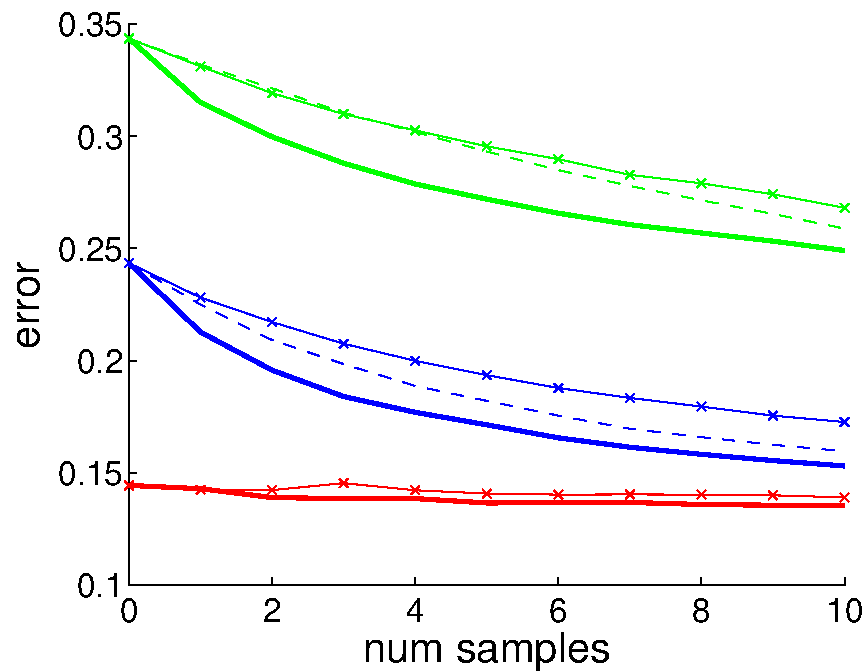
\includegraphics[scale=0.7]{figs/error_syntheticDataLargeScale.pdf}&
          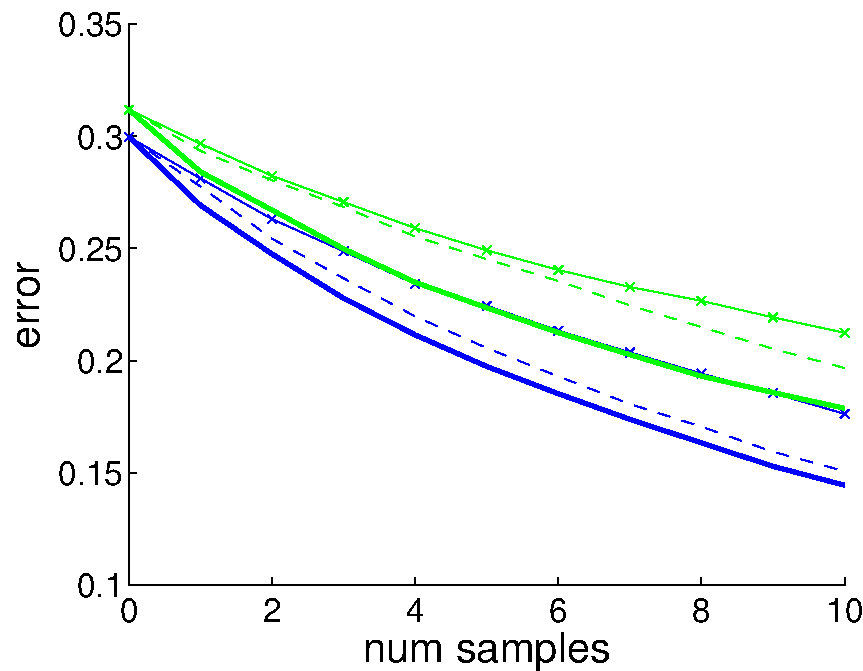
\includegraphics[scale=0.7]{figs/error_sushiDataLargeScale.pdf}&
          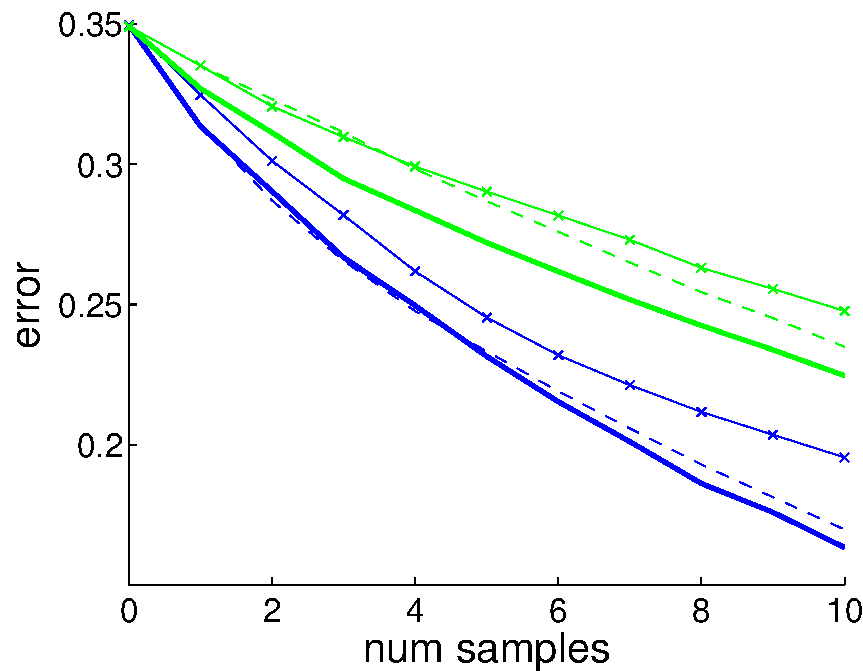
\includegraphics[scale=0.7]{figs/error_movieLensDataLargeScale.pdf}\\
          Election&
          Jura&
          \\
          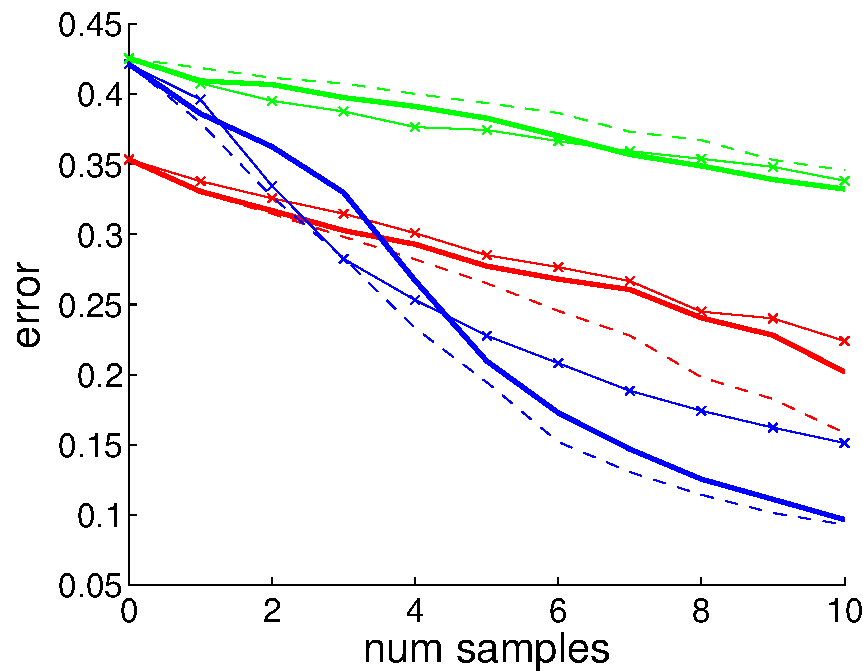
\includegraphics[scale=0.7]{figs/error_electionDataLargeScale.pdf}&
          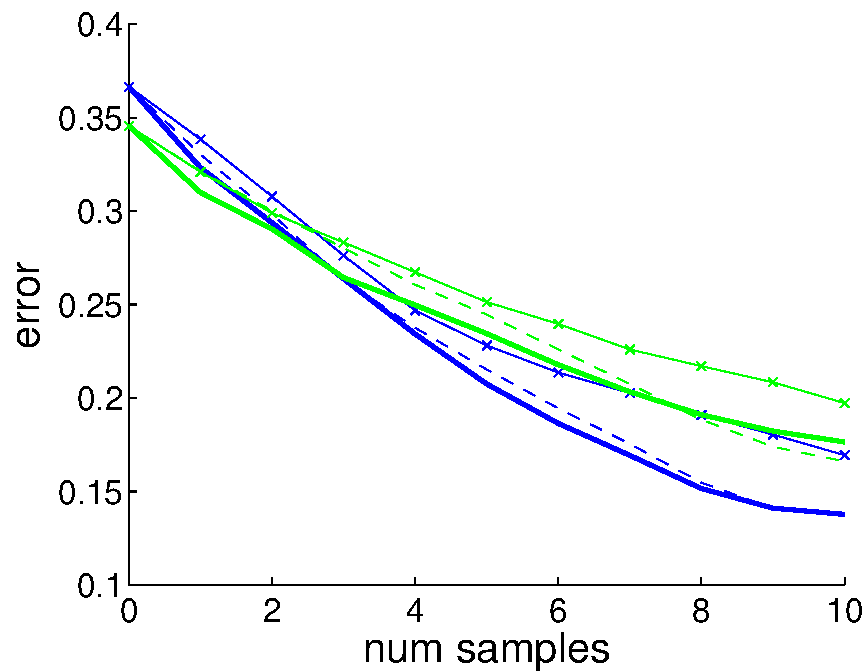
\includegraphics[scale=0.7]{figs/error_juraDataLargeScale.pdf}&
          \hskip1.0cm \raisebox{0.15\height}{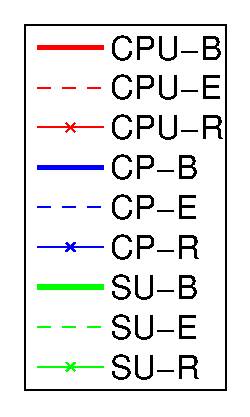
\includegraphics[scale=1.0]{figs/legend.pdf}}
          \end{tabular}
          %}
          \caption{Average test error for CPU, CP and SU, using the strategies BALD (-B), entropy
          (-E) and random (-R) for active learning.
          For clarity, the curves for CPU are included only in the Synthetic and Election datasets.
          The complete plots can be found in Section 10 of the supplementary
          material.\label{fig:learningcurves}}
          \end{figure}
        \end{block}

        \begin{block}{Acknowledgements}
          NH is a recipient of the Google Europe Fellowship in Statistical Machine Learning, and
          this research is supported in part by this Google Fellowship.
          JMH is supported by Infosys Labs, Infosys Limited.
        \end{block}

        \begin{block}{References}
          {\footnotesize
            \bibliographystyle{hippocampus}
            \bibliography{bib/bibliog}
          }
        \end{block}


      \vskip2.5ex
    \end{column}
  \begin{column}{\sepwid}\end{column}			% empty spacer column
 \end{columns}
\end{frame}
\end{document}
